\documentclass[]{article}

\usepackage{graphicx}

%opening
\title{Sensores y circuitos l\'ogicos}
\author{Juan Barbosa}

\begin{document}

\maketitle

\begin{center}
	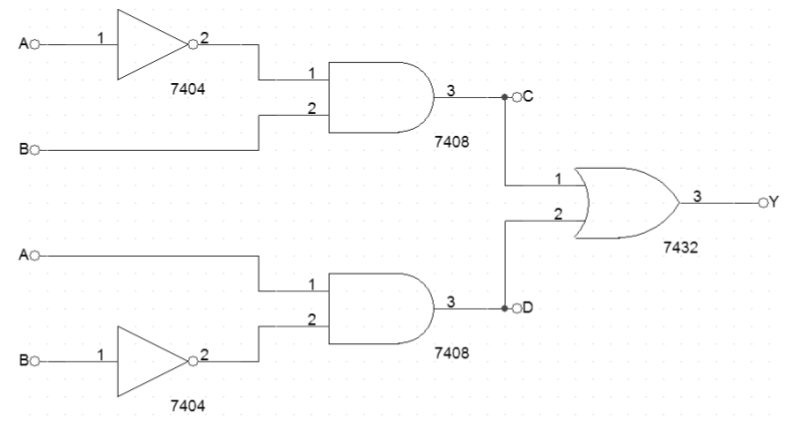
\includegraphics[scale = 0.3]{Circuit.png}
\end{center}

\begin{table}[h]
	\centering
	\begin{tabular}{cc||cccc}
		\hline
		 & & $C = \bar{A} \cdot B$ & $D = A \cdot \bar{B}$ & $Y = C + D$ \\
		\textbf{A} & \textbf{B} & \textbf{C} & \textbf{D} & \textbf{Y} \\
		\hline
		0 & 0 & 0 & 0 & 0 \\
		0 & 1 & 1 & 0 & 1 \\
		1 & 0 & 0 & 1 & 1 \\
		1 & 1 & 0 & 0 & 0 \\
		\hline
	\end{tabular}
\end{table}
\end{document}
